% ============================================================
%  Figure 1 — OACP System Framework
%  Standalone TikZ → compile with: pdflatex fig_framework.tex
%  Then 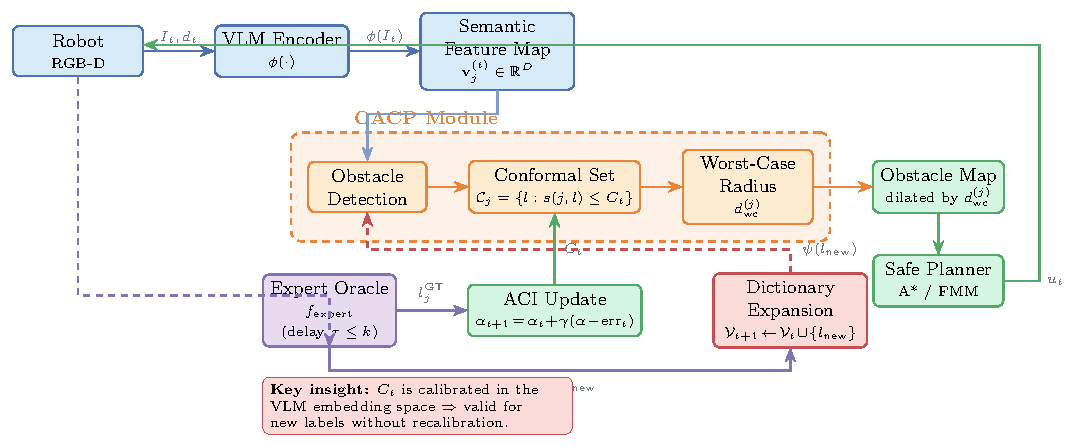
\includegraphics{fig_framework.pdf} in draft.tex
% ============================================================
\documentclass[border=6pt]{standalone}
\usepackage{tikz}
\usetikzlibrary{arrows.meta, positioning, shapes.geometric, fit,
                 decorations.pathreplacing, calc, backgrounds}
\usepackage{amsmath,amssymb}
\usepackage{xcolor}

% ── Colour palette (ICML / NeurIPS style) ──
\definecolor{cBlue}{HTML}{4C72B0}
\definecolor{cOrange}{HTML}{E8853A}
\definecolor{cGreen}{HTML}{55A868}
\definecolor{cRed}{HTML}{C44E52}
\definecolor{cPurple}{HTML}{8172B2}
\definecolor{cGray}{HTML}{6C757D}
\definecolor{cLightBlue}{HTML}{D6EAF8}
\definecolor{cLightOrange}{HTML}{FDEBD0}
\definecolor{cLightGreen}{HTML}{D5F5E3}
\definecolor{cLightRed}{HTML}{FADBD8}
\definecolor{cLightPurple}{HTML}{E8DAEF}

\begin{document}
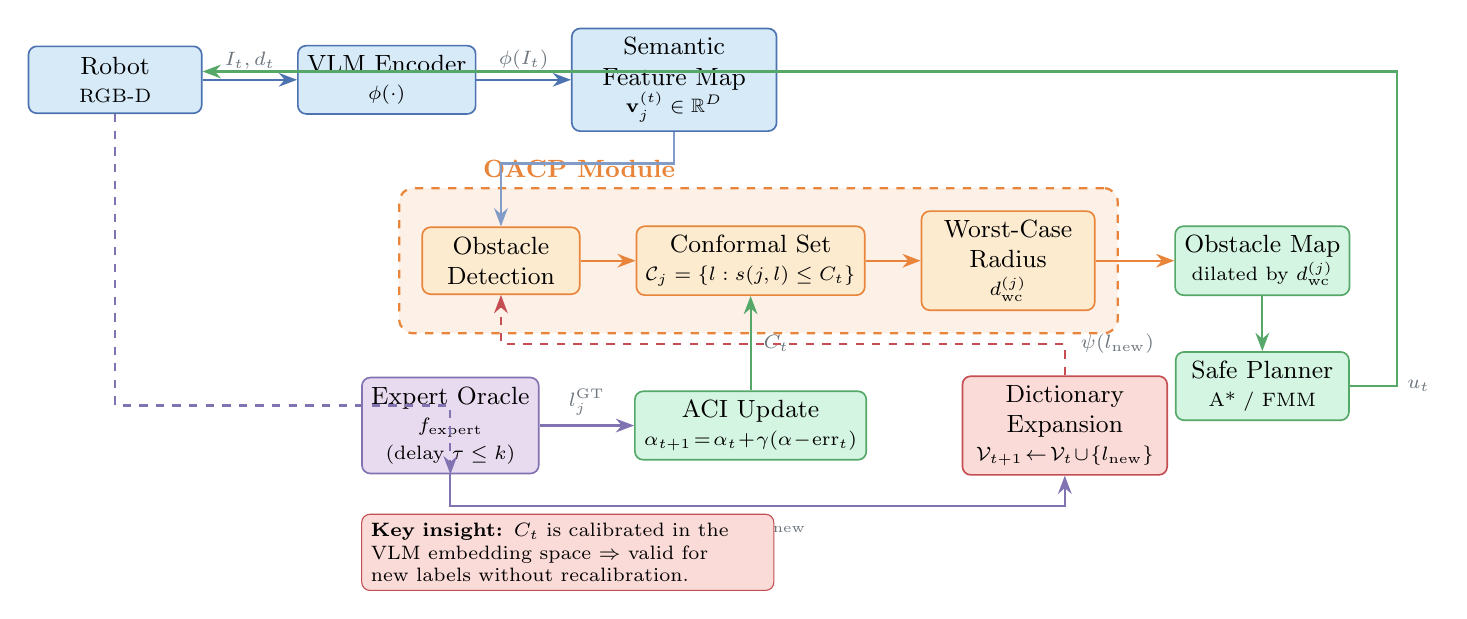
\begin{tikzpicture}[
    >=Stealth,
    node distance=0.6cm and 0.8cm,
    font=\small,
    box/.style={draw, rounded corners=3pt, minimum height=0.85cm,
                minimum width=2.2cm, align=center, line width=0.6pt},
    bigbox/.style={draw, rounded corners=5pt, line width=0.8pt,
                   inner sep=8pt, fill opacity=0.12},
    arr/.style={->, thick, >=Stealth},
    darr/.style={->, thick, >=Stealth, dashed},
    lbl/.style={font=\scriptsize, text=cGray},
]

% ================================================================
%  ROW 1: Perception (left) + Semantic Feature Map (centre)
% ================================================================

\node[box, fill=cLightBlue, draw=cBlue] (robot) {Robot\\[-1pt]{\scriptsize RGB-D}};

\node[box, fill=cLightBlue, draw=cBlue, right=1.2cm of robot] (vlm)
    {VLM Encoder\\[-1pt]{\scriptsize $\phi(\cdot)$}};

\node[box, fill=cLightBlue, draw=cBlue, right=1.2cm of vlm,
      minimum width=2.6cm] (fmap)
    {Semantic\\Feature Map\\[-1pt]{\scriptsize $\mathbf{v}_j^{(t)} \in \mathbb{R}^D$}};

\draw[arr, cBlue] (robot) -- node[above, lbl] {$I_t, d_t$} (vlm);
\draw[arr, cBlue] (vlm)   -- node[above, lbl] {$\phi(I_t)$} (fmap);

% ================================================================
%  ROW 2: OACP Module (centre, highlighted)
% ================================================================

\node[box, fill=cLightOrange, draw=cOrange,
      below=1.2cm of fmap, xshift=-2.2cm, minimum width=2.0cm] (det)
    {Obstacle\\Detection};

\node[box, fill=cLightOrange, draw=cOrange,
      right=0.7cm of det, minimum width=2.4cm] (cset)
    {Conformal Set\\[-1pt]{\scriptsize $\mathcal{C}_j = \{l : s(j,l) \le C_t\}$}};

\node[box, fill=cLightOrange, draw=cOrange,
      right=0.7cm of cset, minimum width=2.2cm] (wc)
    {Worst-Case\\Radius\\[-1pt]{\scriptsize $d_{\mathrm{wc}}^{(j)}$}};

\draw[arr, cOrange] (det) -- (cset);
\draw[arr, cOrange] (cset) -- (wc);

% Feature map → detection
\draw[arr, cBlue!70] (fmap.south) -- ++(0,-0.4) -| (det.north);

% OACP bounding box
\begin{scope}[on background layer]
\node[bigbox, fill=cOrange, draw=cOrange, dashed,
      fit=(det)(cset)(wc),
      label={[font=\small\bfseries, text=cOrange]above left:OACP Module}] (oacpbox) {};
\end{scope}

% ================================================================
%  ROW 3: ACI + Dictionary Expansion
% ================================================================

\node[box, fill=cLightGreen, draw=cGreen,
      below=1.2cm of cset, minimum width=2.6cm] (aci)
    {ACI Update\\[-1pt]{\scriptsize $\alpha_{t+1}\!=\!\alpha_t\!+\!\gamma(\alpha\!-\!\mathrm{err}_t)$}};

\node[box, fill=cLightPurple, draw=cPurple,
      left=1.2cm of aci, minimum width=2.0cm] (expert)
    {Expert Oracle\\[-1pt]{\scriptsize $f_{\mathrm{expert}}$}\\[-1pt]{\scriptsize (delay $\tau \le k$)}};

\node[box, fill=cLightRed, draw=cRed,
      right=1.2cm of aci, minimum width=2.6cm] (dict)
    {Dictionary\\Expansion\\[-1pt]{\scriptsize $\mathcal{V}_{t+1} \!\leftarrow\! \mathcal{V}_t \!\cup\! \{l_{\mathrm{new}}\}$}};

% Expert → ACI
\draw[arr, cPurple] (expert) -- node[above, lbl] {$l_j^{\mathrm{GT}}$} (aci);

% Expert → Dict (novel label)
\draw[arr, cPurple] (expert.south) -- ++(0,-0.4) -| (dict.south)
    node[pos=0.25, below, lbl] {novel $l_{\mathrm{new}}$};

% ACI → conformal set (threshold feedback)
\draw[arr, cGreen] (aci.north) -- node[right, lbl, xshift=1pt] {$C_t$} (cset.south);

% Dict → detection (new labels)
\draw[darr, cRed] (dict.north) -- ++(0,0.4) -| (det.south)
    node[pos=0.0, right, lbl, xshift=2pt] {$\psi(l_{\mathrm{new}})$};

% Robot → Expert (delayed observation)
\draw[darr, cPurple] (robot.south) -- ++(0,-3.7) -| (expert.south);

% ================================================================
%  RIGHT: Planning output
% ================================================================

\node[box, fill=cLightGreen, draw=cGreen,
      right=1.0cm of wc, minimum width=2.2cm] (obsmap)
    {Obstacle Map\\[-1pt]{\scriptsize dilated by $d_{\mathrm{wc}}^{(j)}$}};

\node[box, fill=cLightGreen, draw=cGreen,
      below=0.7cm of obsmap, minimum width=2.2cm] (plan)
    {Safe Planner\\[-1pt]{\scriptsize A* / FMM}};

\draw[arr, cOrange] (wc) -- (obsmap);
\draw[arr, cGreen]  (obsmap) -- (plan);

% Planner → Robot (control loop)
\draw[arr, cGreen] (plan.east) -- ++(0.6,0) |- ([yshift=3pt]robot.east)
    node[pos=0.0, right, lbl] {$u_t$};

% ================================================================
%  Bottom annotation
% ================================================================

\node[draw=cRed, rounded corners=3pt, fill=cLightRed,
      font=\scriptsize, align=left, text width=5.0cm,
      anchor=north west] at ([yshift=-0.5cm]expert.south west)
    {\textbf{Key insight:} $C_t$ is calibrated in the\\
     VLM embedding space $\Rightarrow$ valid for\\
     new labels without recalibration.};

\end{tikzpicture}
\end{document}
